\chapter{Implementation and Results}\label{Implementation and Results}

\section{LOF}
We have used a synthetic 2-D dataset with 3 clusters of varying density to implement and verify LOF.
Dataset description\\
\begin{table}[H]
	\centering
	\caption{2-D Synthetic Dataset description}
	\label{my-label}
	\begin{tabular}{|l|l|}
		\hline
		& \multicolumn{1}{c|}{2-D synthetic dataset} \\ \hline
		\multicolumn{1}{|c|}{n: Data points} & \multicolumn{1}{c|}{1500}                  \\ \hline
		
		\multicolumn{1}{|c|}{d: Dimensions}  & \multicolumn{1}{c|}{2}                     \\ \hline
		\multicolumn{1}{|c|}{c: Clusters}  & \multicolumn{1}{c|}{3}                     \\ \hline
		
		
		
		Noise Points                         & \multicolumn{1}{c|}{50}                                         \\ \hline
	\end{tabular}
\end{table}

\begin{figure}[H]
	\centering
	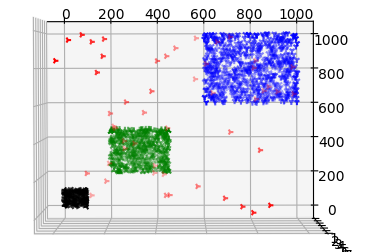
\includegraphics{chap04/LOF_dataset.png}
	\caption{2-D Dataset used for LOF}
\end{figure}

It can be seen from Figure 4.2 that points inside a cluster has LOF values nearly equal to 1 where as noisy points have LOF up to 7. More the LOF score more is the degree of anomaly.

\begin{figure}[H]
	\centering
	\includegraphics{chap04/LOF_result.png}
	\caption{LOF values for synthetic 2-D dataset}
\end{figure}


\section{MiLOF and MiLOF with RKNN}

We have implemented MiLOF and MiLOF with RKNN in two datasets and measured their efficiency.

\subsection{Performance measures}
Simple accuracy and precision is not the correct measure for these unsupervised anomaly detection problems because the two classes, normal and anomalous are not distributed evenly. So to compare their performance, we compare their false positive rate FPR versus true positive rate TPR.

These performance measures are listed below


\[  Precision \, P = \frac{True Positive }{True Positive + False Positive} \]

 \[  Recall \,  R = \frac{True Positive }{True Positive + False Negative} \]

\[  Flase \, Positive \, Rate \,  (FPR) = \frac{False Positive }{False Positive + True Negative} \]
\\
\\
\subsection{Dataset}
\begin{table}[H]
	\centering
	\caption{Dataset Description}
	\label{my-label}
	\begin{tabular}{|c|c|l|}
		\hline
		\multicolumn{1}{|l|}{} & UCI Letter Dataset & UCI PenDigit Dataset \\ \hline
		n: Data points         & 20000              & 10000                \\ \hline
		d: Dimensions          & 16                 & 16                   \\ \hline
		c: Classes             & 26                 & 10                   \\ \hline
	\end{tabular}
\end{table}



\subsection{Results}

\subsubsection{UCI Letter Dataset}

Following are the reults of different performance measure parameters for both the algorithm by varying K and b(available memory) in UCI letter dataset. 



\begin{table}[H]
	\centering
	\caption{MiLOF and MiLOF with RKNN when K changes while b is kept constant}
	
	\label{my-label}
	\begin{tabular}{|c|c|c|c|c|c|c|c|c|}
		\hline
		\multicolumn{1}{|l|}{}    & \multicolumn{4}{c|}{MiLOF}                                                                                                    & \multicolumn{4}{c|}{MiLOF with RKNN}                                                                                          \\ \hline
		\multicolumn{1}{|l|}{K}   & \multicolumn{1}{l|}{Precision} & \multicolumn{1}{l|}{TPR} & \multicolumn{1}{l|}{FPR} & \multicolumn{1}{l|}{TPR/FPR} & \multicolumn{1}{l|}{Precision} & \multicolumn{1}{l|}{TPR} & \multicolumn{1}{l|}{FPR} & \multicolumn{1}{l|}{TPR/FPR} \\ \hline
		\multicolumn{1}{|l|}{100} & 0.132                          & 0.821                              & 0.1154                   & 7.11                         & 0.348                          & 0.727                              & 0.073                    & 9.945                        \\ \hline
		200                       & 0.12                           & 0.874                              & .146                     & 5.96                         & 0.183                          & 0.704                              & 0.076                    & 9.8                          \\ \hline
		300                       & 0.139                          & 0.84                               & 0.1546                   & 5.441                        & 0.255                          & 0.772                              & 0.069                    & 11.561                       \\ \hline
		400                       & 0.184                          & 0.828                              & 0.140                    & 5.88                         & 0.272                          & 0.804                              & 0.821                    & 9.77                         \\ \hline
		500                       & 0.195                          & 0.781                              & 0.157                    & 4.99                         & 0.305                          & 0.761                              & 0.766                    & 9.70                         \\ \hline
		600                       & 0.229                          & 0.772                              & 0.134                    & 5.536                        & 0.355                          & 0.74                               & 0.072                    & 10.252                       \\ \hline
		700                       & 0.221                          & 0.708                              & 0.141                    & 5.01                         & 0.332                          & 0.591                              & 0.067                    & 8.746                        \\ \hline
	\end{tabular}
\end{table}

\begin{figure}[H]
	\centering
	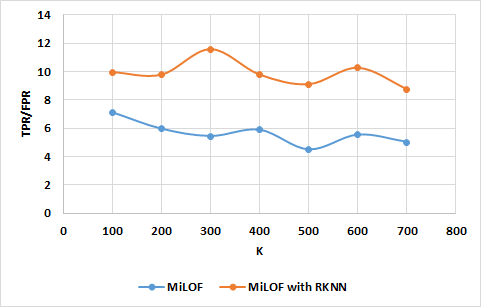
\includegraphics{chap04/varyK.png}
	\caption{TPR/FPR for MiLOF and MiLOF with RKNN when K changes while b is kept constant }
\end{figure}

\begin{table}[H]
	\centering
	\caption{MiLOF and MiLOF with RKNN when b changes while K is kept constant}
	\label{my-label}
	\begin{tabular}{|l|c|c|c|c|c|c|c|c|}
		\hline
		& \multicolumn{4}{c|}{MiLOF}                                                                                                    & \multicolumn{4}{c|}{MiLOF with RKNN}                                                                                          \\ \hline
		b                          & \multicolumn{1}{l|}{Precision} & \multicolumn{1}{l|}{TPR} & \multicolumn{1}{l|}{FPR} & \multicolumn{1}{l|}{TPR/FPR} & \multicolumn{1}{l|}{Precision} & \multicolumn{1}{l|}{TPR} & \multicolumn{1}{l|}{FPR} & \multicolumn{1}{l|}{TPR/FPR} \\ \hline
		2000                       & 0.222                          & 0.707                              & 0.141                    & 5.018                        & 0.332                          & 0.59                               & 0.08                     & 7.35                         \\ \hline
		\multicolumn{1}{|c|}{4000} & 0.291                          & 0.908                              & 0.126                    & 7.215                        & 0.467                          & 0.839                              & 0.054                    & 15.443                       \\ \hline
		\multicolumn{1}{|c|}{5000} & 0.308                          & 0.814                              & 0.103                    & 7.83                         & 0.515                          & 0.856                              & 0.045                    & 18.725                       \\ \hline
		\multicolumn{1}{|c|}{8000} & 0.36                           & 0.915                              & 0.092                    & 9.927                        & 0.67                           & 0.883                              & 0.022                    & 40.89                        \\ \hline
	\end{tabular}
\end{table}


\begin{figure}[H]
	\centering
	\includegraphics{chap04/varyb.png}
	\caption{TPR/FPR for MiLOF and MiLOF with RKNN when b changes while K is constant}
\end{figure}

\subsubsection{UCI Pendigit Dataset}

Following are the reults of different performance measure parameters for both the algorithm by varying K and b(available memory) in UCI pendigit dataset. 

\begin{table}[H]
	\centering
	\caption{MiLOF and MiLOF with RKNN when K changes while b is kept constant}
	\label{my-label}
	\begin{tabular}{|l|c|c|c|c|c|c|c|c|}
		\hline
		& \multicolumn{4}{c|}{MiLOF}                                                                                                    & \multicolumn{4}{c|}{MiLOF with RKNN}                                                                                          \\ \hline
		K                         & \multicolumn{1}{l|}{Precision} & \multicolumn{1}{l|}{TPR} & \multicolumn{1}{l|}{FPR} & \multicolumn{1}{l|}{TPR/FPR} & \multicolumn{1}{l|}{Precision} & \multicolumn{1}{l|}{TPR} & \multicolumn{1}{l|}{FPR} & \multicolumn{1}{l|}{TPR/FPR} \\ \hline
		100                       & 0.618                          & 0.823                              & 0.05                     & 10.98                        & 0.786                          & 0.432                              & 0.0173                   & 24.927                       \\ \hline
		\multicolumn{1}{|c|}{200} & 0.59                           & 0.844                              & 0.099                    & 8.48                         & 0.85                           & 0.463                              & 0.1379                   & 33.569                       \\ \hline
		\multicolumn{1}{|c|}{300} & 0.59                           & 0.783                              & 0.084                    & 9.23                         & 0.773                          & 0.53                               & 0.024                    & 21.748                       \\ \hline
		\multicolumn{1}{|c|}{400} & 0.584                          & 0.7723                             & 0.081                    & 9.455                        & 0.789                          & 0.541                              & 0.0214                   & 25.212                       \\ \hline
		500                       & 0.6203                         & 0.688                              & 0.059                    & 11.628                       & 0.851                          & 0.46                               & 0.011                    & 40.48                        \\ \hline
		600                       & 0.651                          & 0.719                              & 0.045                    & 15.97                        & 0.84                           & 0.67                               & 0.015                    & 44.45                        \\ \hline
		700                       & 0.534                          & 0.739                              & 0.059                    & 12.486                       & 0.797                          & 0.508                              & 0.112                    & 43.65                        \\ \hline
	\end{tabular}
\end{table}



\begin{figure}[H]
	\centering
	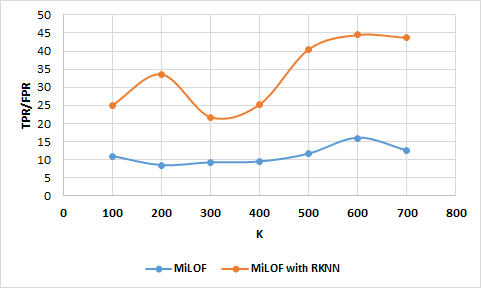
\includegraphics{chap04/varyK2.png}
	\caption{TPR/FPR for MiLOF and MiLOF with RKNN when K changes while b is constant}
\end{figure}



\begin{table}[H]
	\centering
	\caption{MiLOF and MiLOF with RKNN when b changes while K is kept constant}
	\label{my-label}
	\begin{tabular}{|l|c|c|c|c|c|c|c|c|}
		\hline
		& \multicolumn{4}{c|}{MiLOF}                                                                                                    & \multicolumn{4}{c|}{MiLOF with RKNN}                                                                                          \\ \hline
		b                          & \multicolumn{1}{l|}{Precision} & \multicolumn{1}{l|}{TPR} & \multicolumn{1}{l|}{FPR} & \multicolumn{1}{l|}{TPR/FPR} & \multicolumn{1}{l|}{Precision} & \multicolumn{1}{l|}{TPR} & \multicolumn{1}{l|}{FPR} & \multicolumn{1}{l|}{TPR/FPR} \\ \hline
		1000                       & 0.218                          & 0.360                              & .119                     & 3.035                        & 0.1366                         & 0.2158                             & 0.126                    & 1.72                         \\ \hline
		\multicolumn{1}{|c|}{2000} & 0.462                          & 0.412                              & 0.044                    & 9.33                         & 0.471                          & 0.281                              & 0.029                    & 9.678                        \\ \hline
		\multicolumn{1}{|c|}{4000} & 0.5723                         & 0.750                              & 0.052                    & 14.54                        & 0.78                           & 0.65                               & 0.017                    & 38.33                        \\ \hline
		\multicolumn{1}{|c|}{5000} & 0.590                          & 0.794                              & 0.05                     & 15.6                         & 0.79                           & 0.878                              & 0.021                    & 41.22                        \\ \hline
	\end{tabular}
\end{table}

\begin{figure}[H]
	\centering
	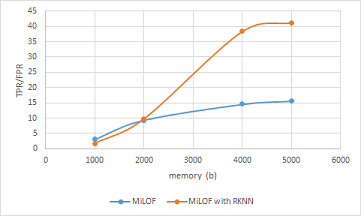
\includegraphics{chap04/varyB2.png}
	\caption{TPR/FPR for MiLOF and MiLOF with RKNN when K changes while b is constant}
\end{figure}